\chapter{Asking Strangers How Much MONEY They Make (Austin, Texas)}

This chapter follows a School of Hard Knocks street interview, curated by LazyingArt LLC, and treats it as a compact lecture on money, structure, and commercial method. We begin with the most socially charged question first, then watch the conversation widen: first to financing, then to team organization, then to networking, risk, asset positioning, and finally to long-horizon financial structure. There is no literal blackboard mathematics here; the formalism is schematic, and its purpose is to preserve the speaker's decision rules without pretending that the interview became a theorem-proof lecture.

\begin{remark}
The equations in this chapter are compact renderings of explicit contrasts, orderings, and transitions stated in the interview. They are not quoted board formulas; they are note-taking devices meant to keep the lecture's logic sharp.
\end{remark}

\section{Opening Hook: Money as a Social Stress Test}

The lecture opens by asking the bluntest possible question: what was the most amount of money someone ever made in a single year? The immediate effect is not information but pressure. We get refusal, hesitation, guarded disclosure, and a small amount of bravado. That is the right opening, because it shows that money is not just an arithmetic topic; it is a topic of status, privacy, and self-presentation.

\begin{equation}
Q_{\mathrm{income}} \longrightarrow \{\text{refusal},\ \text{evasion},\ \text{partial disclosure}\}.
\end{equation}

Only after this pressure test does the host explain the method: the team is moving through downtown Austin, asking strangers about the most money they have made in a year, and using that question as a doorway into a broader discussion of advice, industry, and wealth-building. Even the quick channel introduction matters. The claim that the group built a following of \(1.4\) million gives the interview format its own credential: this is not random street chatter, but a repeated device for extracting commercial self-descriptions under light stress.

\section{Debt, Funding, and First Business Discipline}

The first substantial interview begins with identity. The guest places himself in neurotechnology and describes his business, in his own terms, as getting people off psychiatric medication by means of frequencies and digital frequency patterns. We should preserve that as an attributed claim, not convert it into a scientific proposition. The lecture's real turn comes one question later, when he is asked what he would tell his younger entrepreneurial self.

The answer is immediate and notably unromantic: be careful financially. We do not begin with vision, branding, or scale. We begin with financing discipline.

\begin{equation}
B_{\mathrm{bank}} \prec \{S_{\mathrm{self}},\,F_{\mathrm{friends/family}},\,P_{\mathrm{platforms}}\}.
\end{equation}

Here \(B_{\mathrm{bank}}\) denotes bank borrowing, \(S_{\mathrm{self}}\) self-funding, \(F_{\mathrm{friends/family}}\) capital from aligned relationships, and \(P_{\mathrm{platforms}}\) money raised through contemporary platforms. The point is not a universal theorem about capital structure. The point is that, in this speaker's own accounting, bank debt was his largest regret. He calls it the biggest mistake he ever made.

This ordering matters because the lecture is already teaching us how to rank errors. The upside of borrowed money arrives first in imagination; the downside arrives later in control, pressure, and regret. That is why the advice is not merely ``raise capital,'' but rather: fund it yourself as best you can, and only then widen the circle to people or mechanisms that do not immediately place the bank above the business.

\section{Scaling a Business Through Structure}

From financing, the lecture pivots naturally to a harder question: how does one scale? The speaker answers not with revenue metrics or process charts, but with a distinction between two management geometries.

\begin{definition}
We write \(M_v\) for vertical management and \(M_h\) for horizontal management. In the lecture's own language, \(M_v\) places authority above the group and lets it issue orders downward, whereas \(M_h\) organizes the participants laterally and lets them work together at the same level.
\end{definition}

\begin{align}
M_v &: \text{authority precedes collaboration},\\
M_h &: \text{collaboration precedes authority},\\
M_h + C &\Rightarrow D_{\mathrm{final}}.
\end{align}

The symbol \(C\) denotes a critical moment, and \(D_{\mathrm{final}}\) denotes the final decision pulled by rank. This is the speaker's real refinement: horizontal management is not the abolition of leadership. It is leadership held in reserve until it is needed.

\begin{figure}[h]
\centering

\includegraphics[width=0.72\textwidth]{lecture_113_figure_02.png}
\caption{Visual evidence for the lecture's lateral management picture: the speaker spreads both hands at the same height while describing ``horizontal managers.''}
\end{figure}

The image is important because it gives us the one clear visual artifact in the lecture. There is no drawn chart on a board, but the gesture itself is diagrammatic. The two hands are flat, level, and laterally separated. The subtitle is slightly garbled, but the sense is plain: horizontal managers are not stacked; they are arranged across.

\begin{figure}[h]
\centering
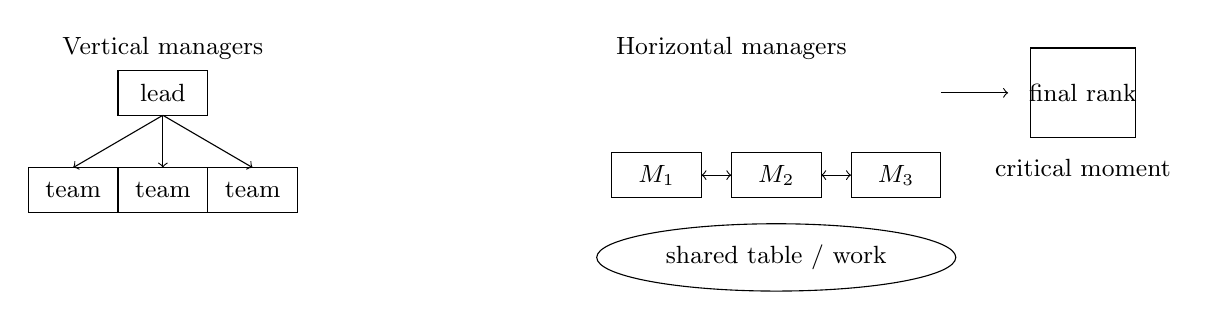
\begin{tikzpicture}[scale=0.95]
\node at (-4.2,3.0) {\small Vertical managers};
\draw (-4.8,2.1) rectangle (-3.6,2.7);
\node at (-4.2,2.4) {\small lead};
\draw (-6.0,0.8) rectangle (-4.8,1.4);
\draw (-4.8,0.8) rectangle (-3.6,1.4);
\draw (-3.6,0.8) rectangle (-2.4,1.4);
\node at (-5.4,1.1) {\small team};
\node at (-4.2,1.1) {\small team};
\node at (-3.0,1.1) {\small team};
\draw[->] (-4.2,2.1) -- (-5.4,1.4);
\draw[->] (-4.2,2.1) -- (-4.2,1.4);
\draw[->] (-4.2,2.1) -- (-3.0,1.4);

\node at (3.4,3.0) {\small Horizontal managers};
\draw (1.8,1.0) rectangle (3.0,1.6);
\draw (3.4,1.0) rectangle (4.6,1.6);
\draw (5.0,1.0) rectangle (6.2,1.6);
\node at (2.4,1.3) {\small \(M_1\)};
\node at (4.0,1.3) {\small \(M_2\)};
\node at (5.6,1.3) {\small \(M_3\)};
\draw[<->] (3.0,1.3) -- (3.4,1.3);
\draw[<->] (4.6,1.3) -- (5.0,1.3);
\draw (4.0,0.2) ellipse (2.4 and 0.45);
\node at (4.0,0.2) {\small shared table / work};

\draw[->] (6.2,2.4) -- (7.1,2.4);
\draw (7.4,1.8) rectangle (8.8,3.0);
\node at (8.1,2.4) {\small final rank};
\node at (8.1,1.4) {\small critical moment};
\end{tikzpicture}
\caption{A cleaned schematic of the lecture's contrast: vertical command, horizontal collaboration, and final rank reserved for a critical moment.}
\end{figure}

\subsection{Question \& Answer}

\paragraph{Question.} How do we scale a business without turning management into pure command-and-control?

\paragraph{Answer.} The lecture's answer is to reverse the default. We do not begin with barking orders and then hope collaboration survives. We begin with shared work, shared vision, and listening. Only when a genuinely critical moment arrives does rank intervene to produce a final decision.

We can write the update rule in the simplest possible form:
\begin{align}
\neg C_t &\Rightarrow \text{remain in } M_h,\\
C_t &\Rightarrow D_{\mathrm{final}} \text{ by rank}.
\end{align}

Once this has been said, the speaker broadens the lesson. Scaling is not merely a matter of process. It is a matter of who surrounds us. The group should be built from professionals, aspiring professionals, or like-minded people in the vision. Then comes the moral clause: we must listen. The lecture is explicit that many people are ready for a fight, ready for the corner, ready to attack. That posture, he says, should not be brought into the business.

\section{Career Breadth, Networking, and Brand}

Before the next long interview, the host briefly resets the frame and reminds us that the Hard Knocks method is to ask everywhere: in line, in stores, around nightlife, in ordinary public motion. This is more than comic relief. It widens the lecture's field. Advice will come not from a podium but from repeated contact with opportunistic strangers.

The next guest is a software-marketing executive. The question is how to break into tech, and the answer is breadth before comfort. He describes taking many opportunities, moving through startups, touching many areas, and learning faster than he would have in a comfortable high-paying role chosen too early. The sequence matters. First comes exposure, then competence, then compensation. Only after that does the lecture ask again about annual peak earnings, yielding the guarded answer of high six figures.

Now the lecture is ready for one of its central tensions. It asks what is more important: who you know or what you know.

\subsection{Question \& Answer}

\paragraph{Question.} Which matters more, who you know or what you know?

\paragraph{Answer.} The lecture does not end with a flat slogan. It first lets the blunt answer stand: who you know matters, and it matters a great deal. Then it qualifies that claim with a deeper rule: network gets us in, but value keeps us there.

\begin{equation}
A_{\mathrm{network}} \xrightarrow{\,V_{\mathrm{provided}}\,} R_{\mathrm{continued}}.
\end{equation}

Here \(A_{\mathrm{network}}\) is access through network, \(V_{\mathrm{provided}}\) is value actually offered, and \(R_{\mathrm{continued}}\) is continued relationship. If one gets into better circles but brings nothing to the table, the process stalls.

\begin{equation}
V_{\mathrm{provided}} = 0 \Rightarrow R_{\mathrm{continued}} \to 0.
\end{equation}

This is the lecture's core correction to the naive networking story. We do not remain in contact with people merely because we met them. We remain in contact when we can offer skill, connection, judgment, or useful work.

A compact rendering of the speaker's logic is:
\begin{align}
A_0 &= \text{entry through network},\\
A_1 &= A_0 + V_{\mathrm{provided}},\\
A_2 &= R_{\mathrm{continued}}.
\end{align}

The same interview adds another important claim: ``you are a brand.'' This means that ordinary social conduct is already economically active. We do not know whom we are about to meet. Even dating platforms, the speaker says, have yielded more business contacts than dates. The larger point is not novelty; it is permeability. Social life and professional opportunity are not sealed compartments.

\section{Risk, Competition, and Personal Conduct}

The middle of the lecture hardens. We move to a business owner in medicine who refuses to disclose the exact amount he made, then grants that it was ``a lot,'' and from there launches into a more severe doctrine of work, risk, and competition. He says plainly that working for oneself is not for everybody. He describes his stem cell company as seventeen years old and doing more than \$4 million in revenue. He identifies himself as someone who always took chances.

What matters here is the order of claims. First: if we sit and wait, we lose. Second: school prestige matters less than many young people think, especially after the first hire. Third: once we are out, the world becomes competitive, and it becomes competitive quickly. The speaker pushes the point almost theatrically: when we enter the market, we are entering against people who have been doing this for decades.

Then the lecture becomes unexpectedly classical. The speaker recalls his father's advice: people buy from people they like. That sentence is easy to trivialize, but in the lecture it does real work. It ties back to networking, to brand, and to the earlier insistence on listening. Likability here is not superficial charm. It is part of commercial trust.

The father's second rule is equally important: do not sweat the small stuff; control the controllables. This turns the section away from swagger and back toward discipline. We cannot govern everything in the field, but we can govern how much noise we let into our decision-making. The lecture thus keeps pairing aggression with self-command. We are asked to take chances, but not to be noisy. We are asked to compete, but not to panic.

\section{Assets, Liquidity, and the Order to Create}

The late lecture pivots from identity and conduct toward portfolio mechanics. A former military interviewee explains that he moved from the military into consulting and project management, while always keeping an entrepreneurial side channel. The concrete mechanism is real estate: at each duty station he would buy a house, and when he moved he would keep the prior house and rent it out. In this way, almost without naming it at first, he became an investor.

\begin{equation}
P_{\mathrm{base\ houses}} \to P_{\mathrm{rentals}} \to (\text{asset rich},\,\text{cash poor}) \to L_{\mathrm{liquid}}.
\end{equation}

This compactly describes the sequence the lecture lays out. Repeated purchases become rentals; rentals become a portfolio; the portfolio creates a balance-sheet condition in which assets are present but cash is tight; and that condition leads to a planned liquidation, motivated by the speaker's expectation that a recession will open better opportunities elsewhere. His own reported annual high is between \$500{,}000 and \$600{,}000, but the more interesting claim is structural: wealth does not merely accumulate; it must sometimes be rearranged.

The next guest, a younger entrepreneur, pushes the lecture toward a more active blueprint. He says that if one wants to be a millionaire, one should create. One should not simply wake up and go with the flow. One should have a plan, live strategically, create a product or channel, fix what is broken, or rework something that already functions well by adding one's own knowledge and spin.

\begin{align}
X_{\mathrm{existing}} &\xrightarrow{\text{own spin + knowledge}} X'_{\mathrm{recreated}},\\
T_{\mathrm{target}} &\to \{c_i\}_{i=1}^{n} \to s_1.
\end{align}

The first line captures the lecture's recreation rule: do not merely copy; alter by knowledge and format. The second line captures the later planning rule: begin with the target business \(T_{\mathrm{target}}\), decompose it into necessary capabilities \(\{c_i\}\), and only then identify the first operational step \(s_1\).

\paragraph{Worked example.} The lecture gives a clean instance of backward planning through the speaker's pool-business example.
\begin{enumerate}
\item Fix the endpoint: suppose the target is a business that builds pools.
\item Decompose the endpoint into trades and capabilities: mechanical work, electrical work, plumbing, gunite, shotcrete, concrete, and the rest of the execution chain.
\item Ask who performs each capability, where they are found, and how good they are.
\item Only after that decomposition decide the first move.
\end{enumerate}

The point is not merely to dream in the direction of a business. The point is to run the arrow backward from the finished operation to the prerequisites that make it possible. That is the lecture's most explicit piece of procedural reasoning.

This section also preserves some of the lecture's sharp quantitative texture. The military investor says he currently has four properties. The younger entrepreneur says he is twenty-eight, started at twenty-one, has two additional businesses, and has made about \$650{,}000 in a single year, while warning that monthly income can swing from \$75{,}000 to \$10{,}000. The notes should keep those numbers because they tell us what kind of volatility the lecture treats as normal.

\section{Buckets, Portability, and the Long Horizon}

The closing movement widens the field again. An LAPD veteran says that at one point he topped \$300{,}000 by doing celebrity weddings and security. The more lasting lesson, however, is his financial advice: invest, diversify, and do not depend only on pension income. He describes a two-bucket structure consisting of pension and deferred compensation.

\begin{equation}
W_{\mathrm{retirement}} = W_{\mathrm{pension}} + W_{\mathrm{deferred\ comp}}.
\end{equation}

We should not make this more technical than the lecture does. No discounting, no optimization, no actuarial analysis. The conceptual point is simple and sound: long-horizon financial stability is strengthened when retirement income is not concentrated in a single channel.

The final interview cools the tone even further. A cybersecurity and privacy professional says that the best decision of his life was to major in engineering. The reason is not that everyone must become an engineer, but that engineering teaches problem solving and therefore opens multiple paths.

\begin{equation}
\text{engineering training} \longrightarrow \text{problem solving} \longrightarrow \text{career optionality}.
\end{equation}

That is an appropriate closing expression for the lecture. It lets the chapter end not on bravado, and not even on income, but on transferability. The interview has moved from the intrusive question of annual money to a calmer question: what kind of training leaves us able to move across industries, roles, and institutional structures without becoming trapped in one narrow identity?

\section{Summary}

The lecture begins by exposing how uneasy people are about money, but it does not stay at the level of confession. It turns that unease into a sequence of rules. First, be careful with financing, especially with bank debt. Second, scale by collaboration first and authority second. Third, network is real, but only value sustains it. Fourth, risk matters, yet so do likability and control of the controllables. Fifth, assets and liquidity are not the same thing, and creation is not the same thing as copying. Finally, wealth can be built not only through entrepreneurial bursts, but also through durable structures such as retirement buckets and portable problem-solving skill.

That sequence is the chapter's real mathematics: not symbols on a board, but a disciplined ordering of choices, constraints, and transitions.